\def\mytitle{MATRICES USING PYTHON}
\def\myauthor{THOUTU RAHUL RAJ}
\def\contact{rdj4648@gmail.com}
\def\mymodule{Future Wireless Communication (FWC)}
\documentclass[10pt, a4paper]{article}
\usepackage[a4paper,outer=1.5cm,inner=1.5cm,top=1.75cm,bottom=1.5cm]{geometry}
\twocolumn
\usepackage{graphicx}
\graphicspath{{./images/}}
\usepackage[colorlinks,linkcolor={black},citecolor={blue!80!black},urlcolor={blue!80!black}]{hyperref}
\usepackage[parfill]{parskip}
\usepackage{lmodern}
\usepackage{amsmath,amsfonts,amssymb,amsthm}
\usepackage{tikz}
	\usepackage{physics}
%\documentclass[tikz, border=2mm]{standalone}
\usepackage{karnaugh-map}
%\documentclass{article}
\usepackage{tabularx}
\usepackage{circuitikz}
\usetikzlibrary{calc}
\usepackage{amsmath}
\usepackage{amssymb}
\renewcommand*\familydefault{\sfdefault}
\usepackage{watermark}
\usepackage{lipsum}
\usepackage{xcolor}
\usepackage{listings}
\usepackage{float}
\usepackage{titlesec}
\providecommand{\norm}[1]{\left\lVert#1\right\rVert}
\providecommand{\sbrak}[1]{\ensuremath{{}\left[#1\right]}}
\providecommand{\lsbrak}[1]{\ensuremath{{}\left[#1\right.}}
\providecommand{\rsbrak}[1]{\ensuremath{{}\left.#1\right]}}
\providecommand{\brak}[1]{\ensuremath{\left(#1\right)}}
\providecommand{\lbrak}[1]{\ensuremath{\left(#1\right.}}
\providecommand{\rbrak}[1]{\ensuremath{\left.#1\right)}}
\providecommand{\cbrak}[1]{\ensuremath{\left\{#1\right\}}}
\providecommand{\lcbrak}[1]{\ensuremath{\left\{#1\right.}}
\providecommand{\rcbrak}[1]{\ensuremath{\left.#1\right\}}}
\newcommand{\myvec}[1]{\ensuremath{\begin{pmatrix}#1\end{pmatrix}}}
\let\vec\mathbf
\providecommand{\mtx}[1]{\mathbf{#1}}
\titlespacing{\subsection}{1pt}{\parskip}{3pt}
\titlespacing{\subsubsection}{0pt}{\parskip}{-\parskip}
\titlespacing{\paragraph}{0pt}{\parskip}{\parskip}
\newcommand{\figuremacro}[5]

\begin{document}

\title{\mytitle}
\author{\myauthor\hspace{1em}\\\contact\\FWC22008\hspace{6.5em}IITH\hspace{0.5em}\mymodule\hspace{6em}ASSIGN-4}
\date{}
	\maketitle
		
	\tableofcontents
\vspace{5mm}
   \section{Problem}
\textbf{ If diagonals of a parallelogram are equal then show that it is a rectangle }
 \section{Construction}
 	\begin{center}
     Figure of Construction
     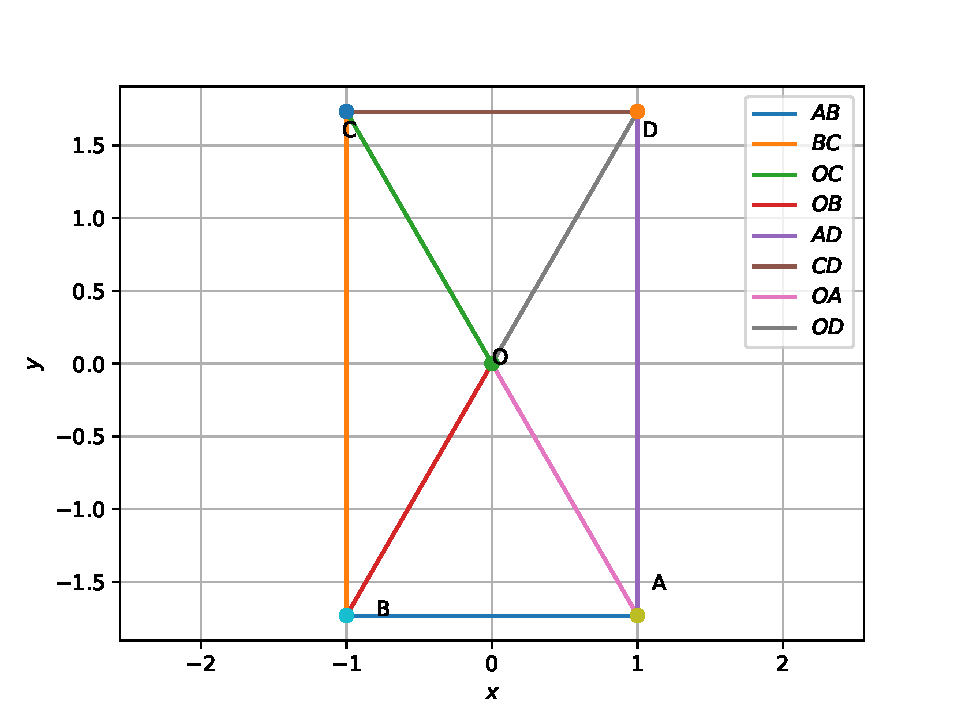
\includegraphics[scale=0.5]{fig.pdf} 
  	\end{center}
  	The input parameters for this construction are 
\begin{center}
\begin{tabular}{|c|c|c|}
	\hline
	\textbf{Symbol}&\textbf{Value}&\textbf{Description}\\
	\hline
	r&6&AC\\
	\hline
	k&4&AB\\ 
	\hline
	${\theta}$& arccos(k/r)&$ \angle $AC\\
	\hline
	\textbf{A}&$\
	\begin{pmatrix}
		0 \\
		0 \\
	\end{pmatrix}$
	&Point A\\
	\hline
	
\end{tabular}
\end{center}

   \section{Solution}

\vspace{1mm}
\textbf{Termux commands :}
\begin{lstlisting}
python3 matrixline.py
\end{lstlisting}


\vspace{.25 cm}
\textbf{To Prove:}
ABCD is a rectangle

 Given:
 ABCD is a parallelogram
\begin{align}
 \vec{B} - \vec{A}= \vec{C}-\vec{D}\
	\end{align}
	And, Diagonals of the parallelogram are equal.
\begin{align}
 \norm{\vec{C} - \vec{A}}^2= \norm{\vec{D}-\vec{B}}^2\
	\end{align}
 	Now, we should prove that its a rectangle i.e
\begin{align}
 \theta = 90
\end{align} 	
 \begin{align}
 \cos \theta_1 =\frac{\mathbf{(A-B)}^T  \mathbf{(B-C)}}{\norm{\vec{(A-B)}}\norm{\vec{(B-C)}}}
 \end{align}
\begin{align}
\brak{\vec{A}-\vec{B}}^T
\brak{\vec{B}-\vec{C}} = 0
\\
\end{align}
from equation (2) 
\begin{align*}
 \norm{\vec{C} - \vec{A}}^2= \norm{\vec{D}-\vec{B}}^2\\
 \norm{{(\vec{A-B}) + (\vec{B-C})}}^2 = \norm{{(\vec{A-B}) + (\vec{B-C})}}^2\\
\end{align*}
After resolving the above equation 
\begin{align}
2(\vec{A}-\vec{B})^T (\vec{B}-\vec{C})=2(\vec{C}-\vec{D})^T (\vec{B}-\vec{C}) 
\end{align}
according to parallelogram theorem, we can write C - D =-(A - B)
\begin{align}
2(\vec{A}-\vec{B})^T (\vec{B}-\vec{C})=-2(\vec{A}-\vec{B})^T (\vec{B}-\vec{C}) \\
2(\vec{A}-\vec{B})^T (\vec{B}-\vec{C})+2(\vec{A}-\vec{B})^T (\vec{B}-\vec{C}) =0 \\
2(\vec{A}-\vec{B})^T (\vec{B}-\vec{C})=0\\
(\vec{A}-\vec{B})^T (\vec{B}-\vec{C})=0
\end{align}
\begin{align}
\implies cos\theta = 0\\
\theta = 90
\end{align}
 	
$\therefore$ It is a rectangle

\vspace{1mm}
The below python code realizes the above construction:	\\
\url{https://github.com/Rahulraj00/Assignments/tree/main/Assignments/assg_4}
\bibliographystyle{ieeetr}
\end{document}